\documentclass[10pt, twocolumn]{revtex4}

\usepackage{times}

\usepackage[a4paper, left=1.85cm, right=1.85cm,
 top=1.85cm, bottom=1.85cm]{geometry}

\usepackage[font=small,
labelfont=bf]{caption}

\usepackage{graphics,graphicx,epsfig,float}
\usepackage{amsmath}

\usepackage{natbib}

\usepackage{dblfloatfix, afterpage}

\usepackage{etoolbox}
\makeatletter
\patchcmd{\frontmatter@RRAP@format}{(}{}{}{}
\patchcmd{\frontmatter@RRAP@format}{)}{}{}{}
\renewcommand\Dated@name{}
\makeatother

\usepackage{fancyhdr}

\def\bibsection{\section*{\refname}}

\pagestyle{fancy}
\renewcommand{\headrulewidth}{0pt}
\lhead{R. Schofield}
\rhead{CMP}

\graphicspath{{figures/}}

\usepackage[none]{hyphenat}


\begin{document}


\title{Small-field Anisotropic Magnetoresistance of a Permalloy Thin Film Oriented Parallel and Perpendicular to the Magnetic Field }
\date{Submitted: \today{}, Date of Experiment: 21/01/19 - 15/03/19}
\author{R. Schofield}
\affiliation{\normalfont Condensed Matter Physics, Epiphany Term}


\begin{abstract}
\section*{Abstract}

Abstract\\
Abstract\\
Abstract\\
Abstract


\end{abstract}

\maketitle
\thispagestyle{plain}


\section{Introduction}

Magnetoresistance is when an applied magnetic field causes the internal resistance of a material to increase. In particular, Anisotropic Magnetoresistance (AMR) is when the resistance increase is dependent upon the angle between the material and the applied magnetic field. It was first discovered by Lord Kelvin in 1856.\cite{kelvinXIXElectrodynamicQualities1857} A further study was done in 1975 which defined the angular dependence of the AMR induced resistance
\begin{equation}
\rho(\theta) = \rho_\perp + (\rho_\parallel - \rho_\perp)cos^2(\theta)
\end{equation}
where $\rho(\theta)$ is the measured resistance, $\rho_\perp$ is the resistance with the field perpendicular to the current, and $\rho_\parallel$ is the resistance with the field parallel to the current.\cite{mcguireAnisotropicMagnetoresistanceFerromagnetic1975} The origin  of the AMR effect is in spin orbit coupling.\cite{Campbell_1970} %can expand this is necessary


\section{Method}

In this experiment we used a 500\AA{} thin film of permalloy as our sample. Permalloy is an alloy composed of 80\% nickel and 20\% iron. We chose this material due to the significant magnetic properties it possesses, including a strong AMR. \\
\\
We mounted our sample, a hall probe and a platinum thermometer to a probe and inserted the probe into a cryostat under a magnetic field as shown.

\begin{figure}[H]
	\centering
	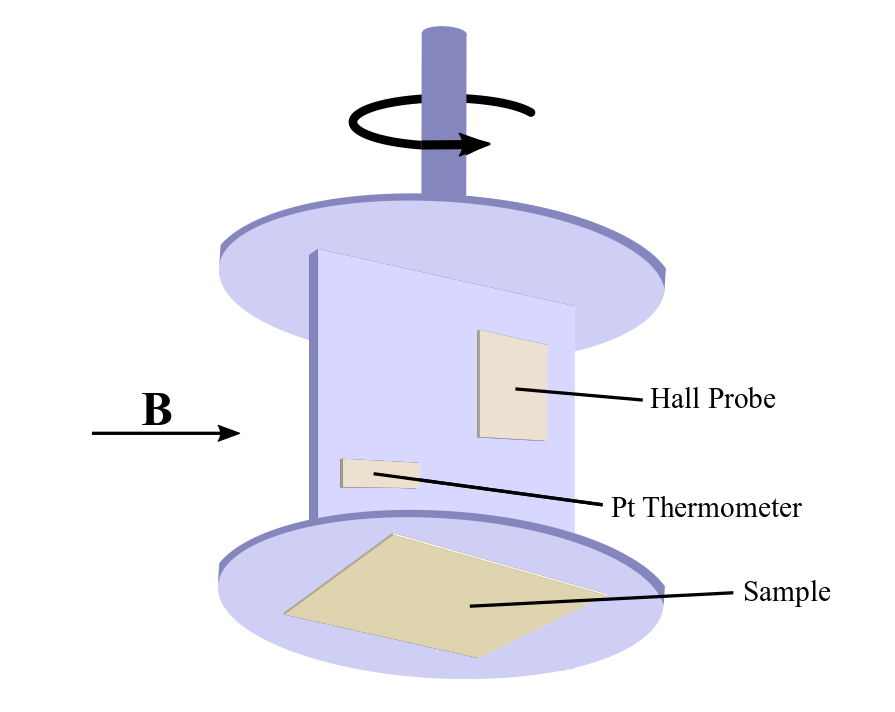
\includegraphics[width = \columnwidth]{drawing.png}
	\caption{Diagram of setup.  The sample is initially mounted perpendicular to the hall probe and thermometer, so that the largest faces are parallel to the direction of the magnetic field.}
	\label{fig:setup1}
\end{figure}

This setup will be referred to as the horizontal mount. The vertical mount has the hall probe and platinum thermometer in the same position, and the sample mounted to the opposite face of the same part of the probe.\\
\\
The sample and hall probe were both wired with a four point measurement. The platinum thermometer could only support two contacts, so for this a pseudo-four-point measurement was used. The four point or Kelvin method of measurement employs two pairs of contacts, one within the other. 

\begin{figure}[H]
	\centering
	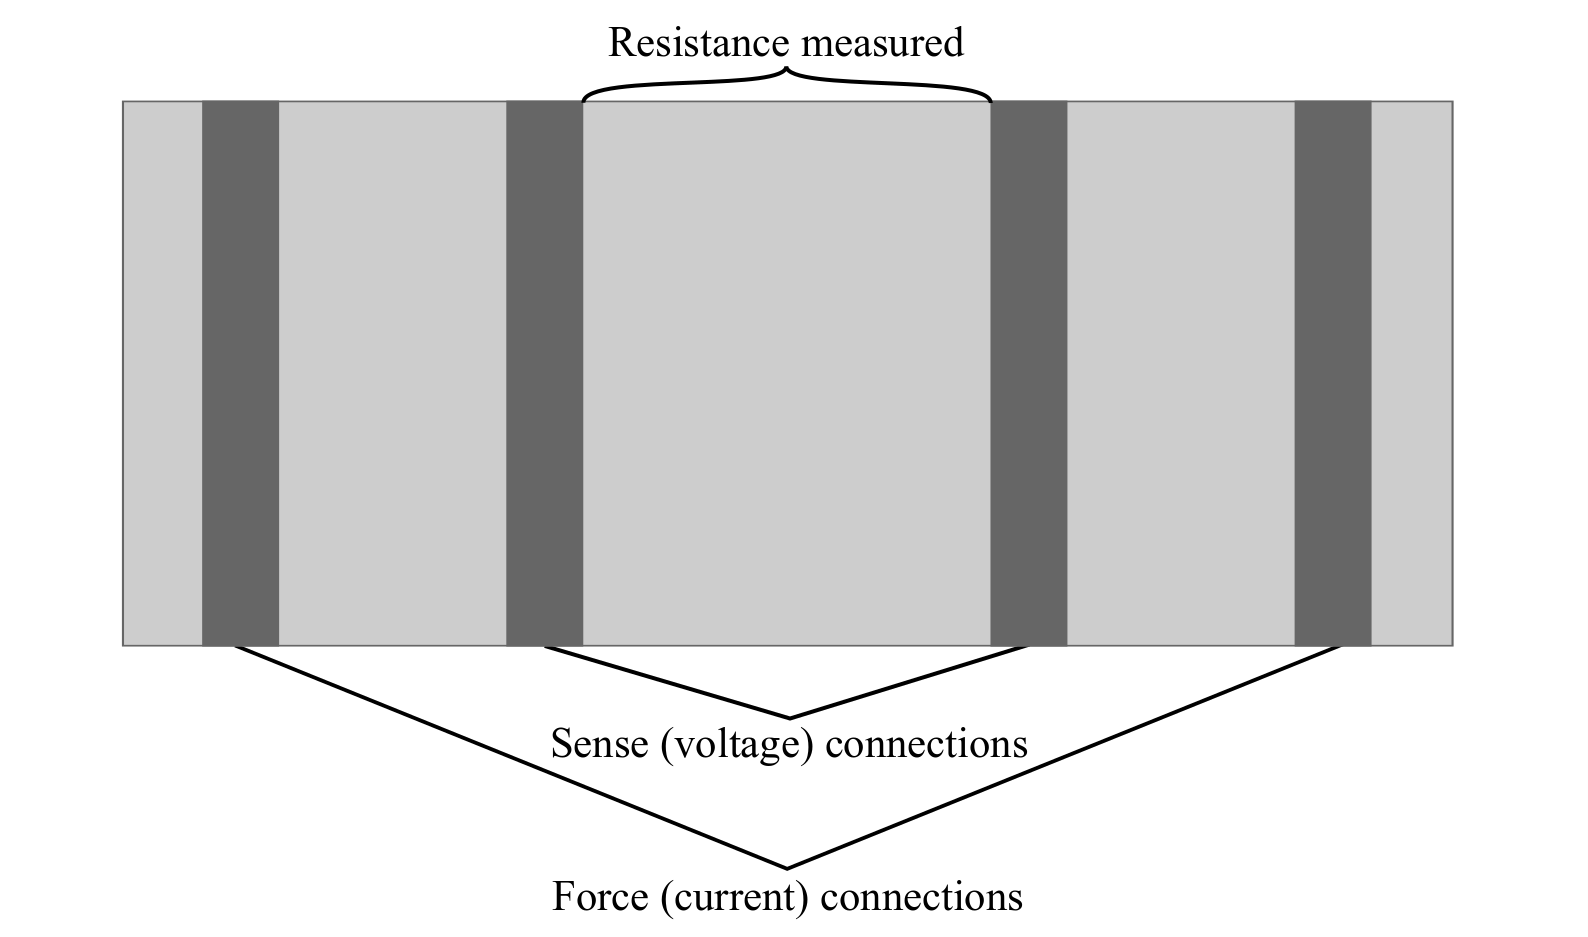
\includegraphics[width = \columnwidth]{drawing-1.png}
	\caption{Diagram of the connections on the sample. The connections were made by using silver paint to connect wires to the sample along the lines shown.}
	\label{fig:setup2}
\end{figure}

The outer pair of contacts supply a low 'driving' current to the sample while the inner pair measure the voltage. By measuring the current and voltage in this way the error caused by the resistance in the wires is negligible.\\ %could explain more?
\\
The strength of the magnetic field passing through the probe was varied by controlling the current input to the electromagnet. Intervals of 0.05A were used, which corresponds to *** T. At each magnetic field strength we rotated the probe one full rotation, taking measurements at small intervals of approximately 10-15 degrees. Because we were manually rotating the sample we could not make the intervals more precise, but this uncertainty does not contribute to the final errors as we used the hall probe measurements to calculate the angle of each measurement. \\
\\
Initially we took measurements at room temperature. Then we filled the cryostat with liquid nitrogen, causing the chamber to be maintained at the boiling point of nitrogen, 77.2K.\\ %more specific and errors 
\\
In order to find the angle between the plane of the sample and the magnetic field, we measured the maximum and minimum values of the hall probe resistance during a full rotation. We then used this data to fit the measured hall probe readings to a cosine curve, as the magnitude of the hall probe resistance is greatest when the magnetic flux passes through the greatest area of the probe - at 0 and 180 degrees - and follows a cosine curve as the probe rotates. We then used this fit to extrapolate the angles for each measurement.


\section{Results}

\begin{figure}[H]
	\centering
	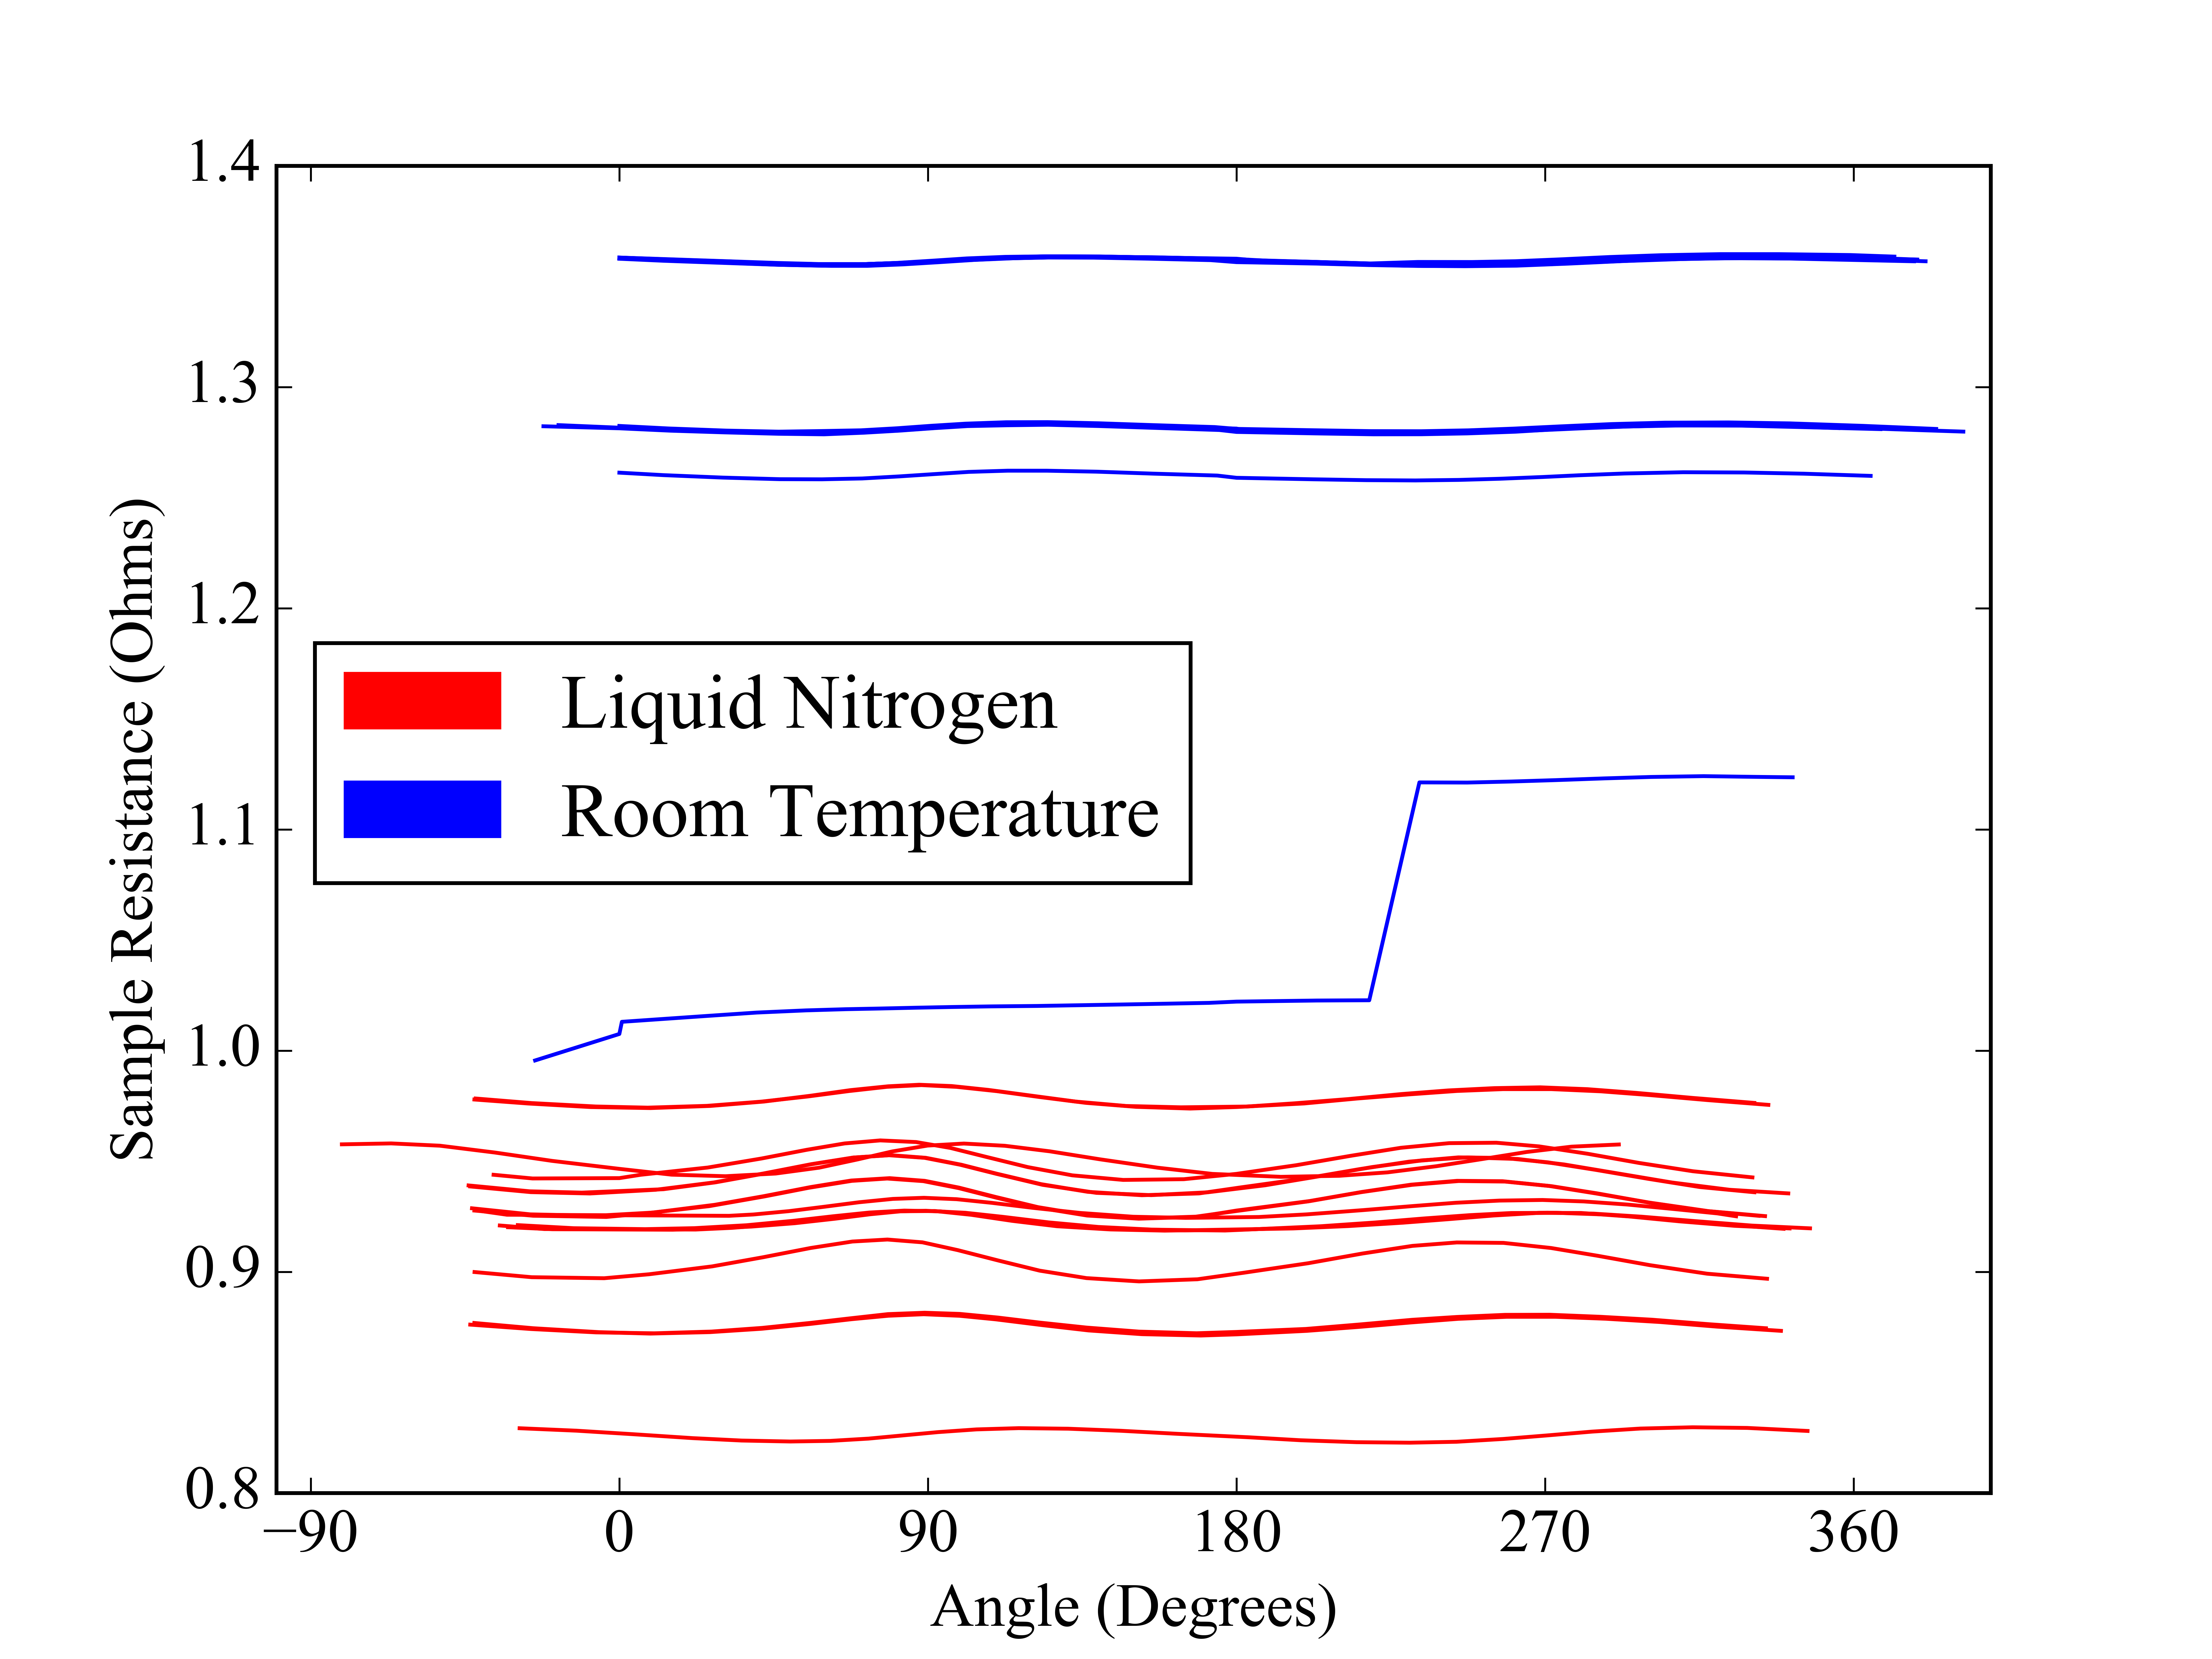
\includegraphics[width = \columnwidth]{LNRTfig.png}
	\caption{Graph of sample resistance against angle with magnetic field at both Liquid Nitrogen Temperature ($\approx$77K) and Room Temperature ($\approx$300K). Magnetic field strength varied from (0-0.75) at both temperatures.}
	\label{fig:horiz_all}
\end{figure}

As expected, the sample resistance was significantly lower when cooled with liquid nitrogen than at room temperature. The room temperature measurements were mostly split into two groups, which we found to be the two different days these measurements were taken over. There were also two further sets of data which did not fit into these two groups.\\ %***check temp for anomalies***
\\
\begin{figure}[H]
	\centering
	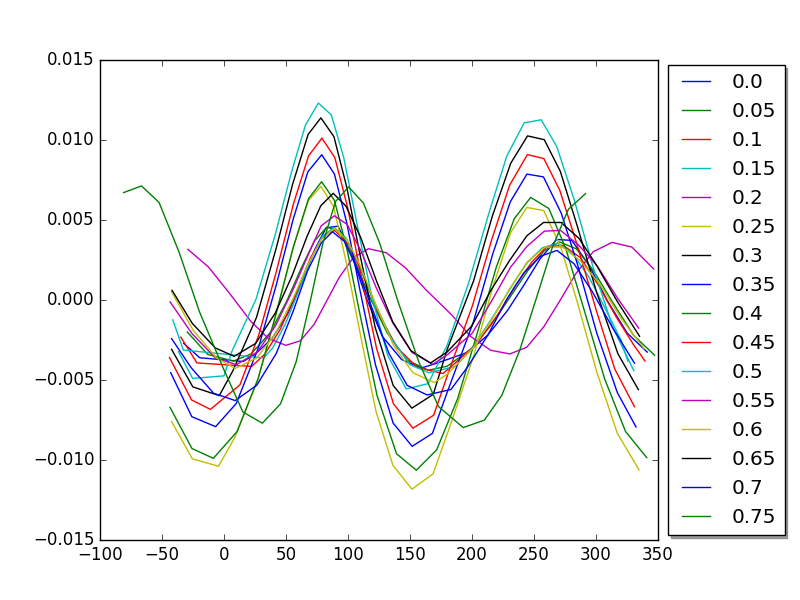
\includegraphics[width = \columnwidth]{LN_adj_fig.png}
	\caption{LN close up of shape, magnitude against current split}
	\label{fig:horiz_LN}
\end{figure}

\begin{figure}[H]
	\centering
	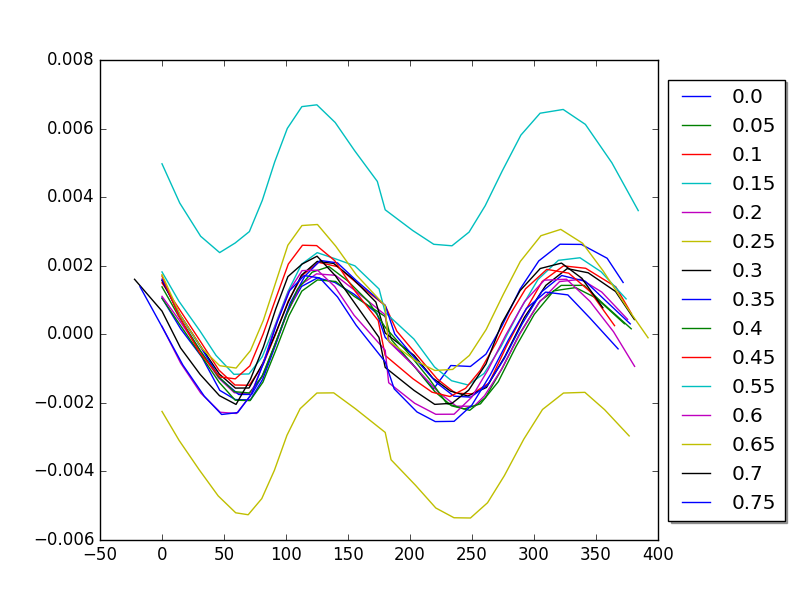
\includegraphics[width = \columnwidth]{RT_adj_fig.png}
	\caption{RT close up of shape, magnitude against current split. 0.5A removed}
	\label{fig:horiz_RT}
\end{figure}

%amplitude against current for both - fit with offset?
Figures ~\ref{fig:horiz_LN} and ~\ref{fig:horiz_RT} are plotted with a vertical offset so that for each set of data, the value of the resistance is zero at 90 degrees. This is because 90 degrees is when the magnetic field strength is at a minimum and therefore the easiest angle to locate (most accurate?). This offset was included because otherwise in order for the y axis to be sufficiently large to fit the plots on one graph the wave behaviour is compressed to the extent that it is not visible.

Both room temperature and liquid nitrogen temperatures produced the expected AMR angular dependence with a $cos^2$ shape. At room temperature there was no clear trend between  AMR magnitude increase with magnetic field, but at liquid nitrogen temperature the amplitude of the curve visibly increased with magnetic field strength. The room temperature data also appears to have a negative skew, while the majority of the liquid nitrogen data does not.\\
\\
\begin{figure}[H]
	\centering
	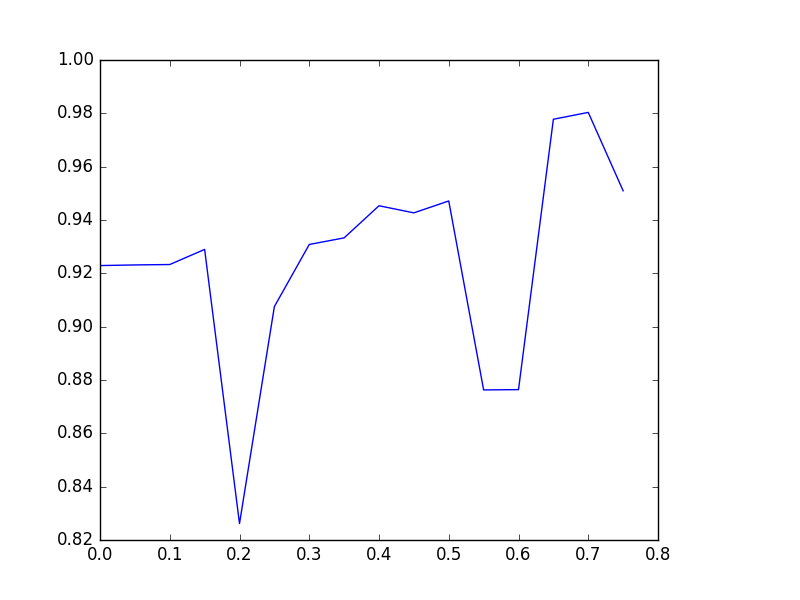
\includegraphics[width = \columnwidth]{LN_offsets.png}
	\caption{LN offset against current}
	\label{fig:horiz_LN_offset}
\end{figure}

\begin{figure}[H]
	\centering
	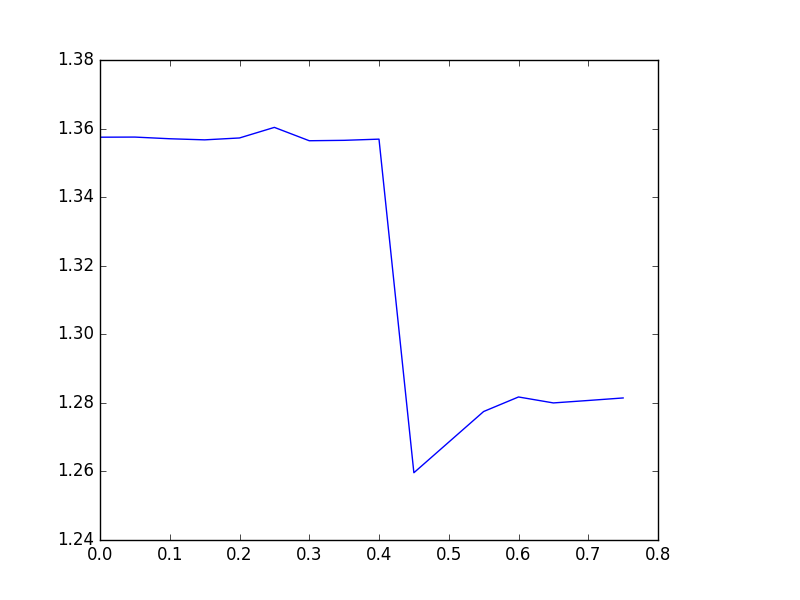
\includegraphics[width = \columnwidth]{RT_offsets.png}
	\caption{RT offset against current 0.5A removed}
	\label{fig:horiz_RT_offset}
\end{figure}

For the room temperature measurements, the offset seems to be constant, with the discrepancies corresponding to different temperatures on different days. At liquid nitrogen temperature however, there seems to be a positive correlation overall between magnetic field strength and offset.\\  %***should offset be from low point??? is this possible?

%Plot amplitude against current - same graph?
%calculate AMR percentage
%calculate perpendicualar and parallel resistances, use this to test original equation. graph?

\begin{figure}[H]
	\centering
	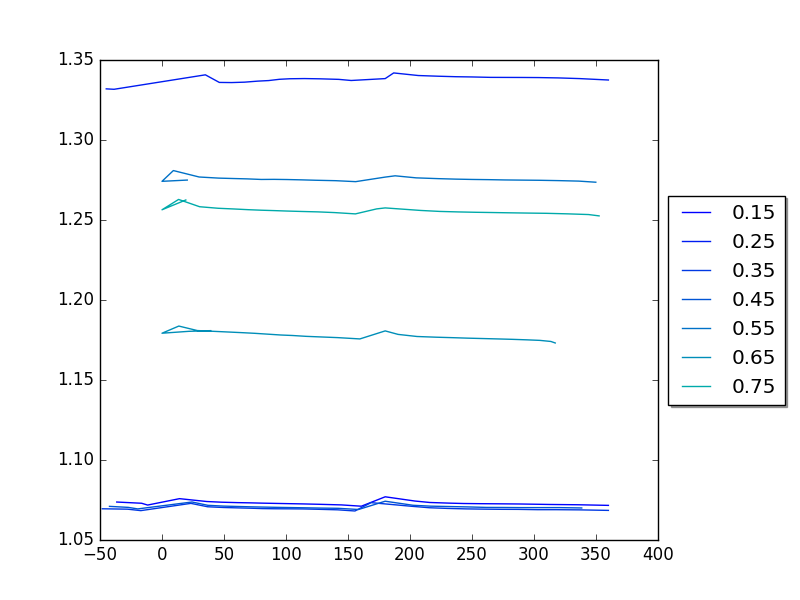
\includegraphics[width = \columnwidth]{Vert_plot.png}
	\caption{RT vert}
	\label{fig:vert_all}
\end{figure}

\begin{figure}[H]
	\centering
	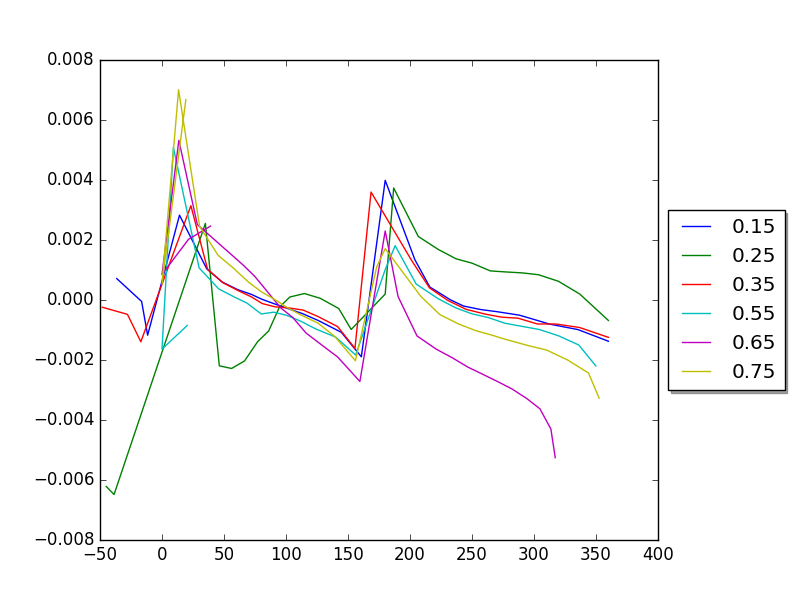
\includegraphics[width = \columnwidth]{RT_adj_fig_vert.png}
	\caption{RT vert close up of shape, magnitude against current split}
	\label{fig:vert_RT}
\end{figure}

Figure ~\ref{fig:vert_RT} is plotted with a vertical offset in the same way as Figures ~\ref{fig:horiz_LN} and ~\ref{fig:horiz_RT}. In the vertical mount configuration, rather than a smooth $cos^2$ shape the resistance instead showed two sharp peaks, one at approximately 0 degrees and one at 180 degrees. 

\begin{figure}[H]
	\centering
	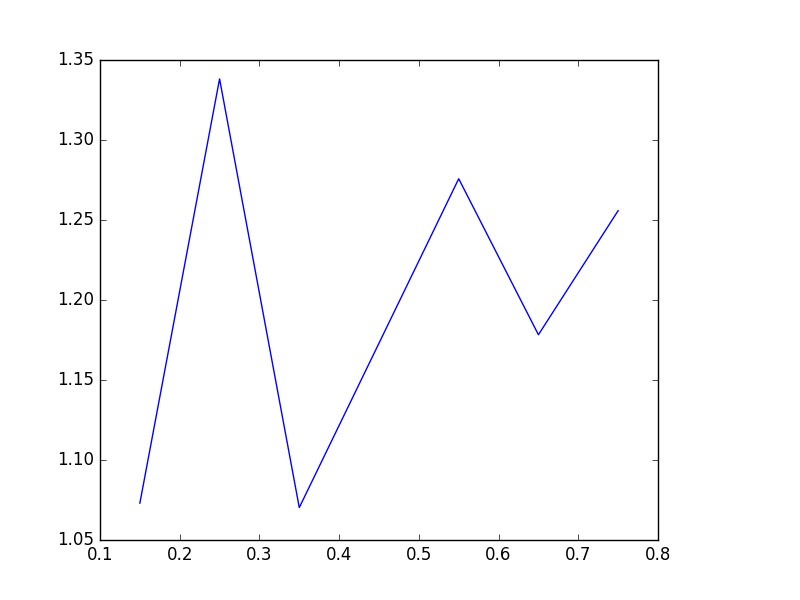
\includegraphics[width = \columnwidth]{Vert_RT_offsets.png}
	\caption{RT vert offset}
	\label{fig:vert_RT_offsets}
\end{figure}

The offsets were within the same range as for the horizontal mount, but showed no apparent increase. Instead they appeared to oscillate about a value lower than any offset for the horizontal mount. %fit and quantify? %amplitudes


\section{Discussion}

There were several sets of data that appeared anomalous, the most obvious of which was the room temperature measurement with the magnet current set to 0.5A. This data has a significantly lower resistance than the other room temperature measurements, and shows a sudden increase in resistance between 219 and 233 degrees. There is no significant change in driving current, temperature reading from the platinum thermometer, or field strength reading from the hall probe that would explain this anomaly. It is most likely that it was caused by a problem with the experimental setup - this data set was taken after the others, and the wiring may have become loose or damaged such that as the probe was turned the measurements were significantly altered ***(bad wording). This would also explain the unusually low overall resistance, as the temperature readings did not differ from the other room temperature measurements enough to cause this drop. \\
\\
The temperature varied more than expected between days while taking the room temperature measurements, which meant that we could not directly compare the data between days. We had assumed that the building's heating system would keep the room temperature constant, but it would have been more prudent to heat the sample to a constant temperature slightly above room temperature so that we could control the temperature with the heater and thus maintain it more accurately. \\
\\
skew?\\
\\
The increase of the overall resistance measured at liquid nitrogen temperature with magnetic field strength may be due to a small heating effect caused by the magnetoresistance. \\
\\
In our experiment, we had to rotate the probe manually which caused the error on the calculated angle to be large. Given the appropriate equipment, it would have been far more accurate to automate the rotation of the probe so that it was rotated by a precise angle each time. This would mean that the error on the angle would be the equipment error only rather than the standard error from fitting the hall probe data to a curve and extrapolating angles.\\
\\
difference between mounts?\\
\\
***Is vertical mount still cos squared? Calculate from parallel and perpendicular resistances.\\
\\
It could be inferred from the difference between the horizontal and vertical mount data that the magnitude of the AMR effect at a particular orientation is proportional to either the distance over which the magnetic field passes through the sample or the surface area of the sample that is in the plane of the magnetic field. \\
\\
In our experiment, we were unable to take data for the vertical mount under liquid nitrogen cooling due to time constraints. Since the AMR effect is smaller at higher temperatures, this meant we were unable to draw any conclusions about the effect of the magnetic field strength on the magnitude of the AMR effect. As can be seen in the horizontal mount data, the difference between different magnetic field strengths is not visible at room temperature, but is clear when the sample is cooled with liquid nitrogen. It is likely that the same is true with the vertical mount.\\
\\

\section{Conclusions}

Our experiment using the horizontal mount concurred with previous findings that the resistance of a sample exhibiting AMR varies as a $cos^2$ curve. The AMR effect was more pronounced when cooled using liquid nitrogen, and when magnetic field strength was increased.


\bibliographystyle{abbrv}

\bibliography{My_Library.bib}

\newpage


\section{Appendix}

Error appendix\\
\\
Error on voltage and current to error on resistance\\
\\
hall probe error to angle error\\
\\
fit line residuals?\\
\\
Thermometer calibration error\\
\\
\end{document}
